This chapter describes how to simulate from our multiGLMM for clustered
competing risks data, and describes a real-based dataset used as an
application example. The simulation procedure is addressed in
\autoref{cap:simu}. In \autoref{cap:data} a simulated dataset based on
the Nordic Cancer Union (NCU) twins data is presented as an application
example.

\section{SIMULATING FROM A \(\text{multiGLMM}\) FOR THE CIF OF CLUSTERED
  COMPETING RISKS DATA}
\label{cap:simu}

Being able to simulate data from a model is a key task, fundamental to
assess the finite-sample properties and the estimation procedure of a
given statistical model. Since our model is very similar and was based
on the one proposed by \citeonline{SCHEIKE}, in the first moment the
idea was to follow the same guidelines proposed by them. However, after
an extensive period of thought, we reached the conclusion that they are
not really simulating from the model. Instead of using the proposed
framework to generate the failure probabilities, they use just a piece
of that. Besides, with the excuse of being controlling the censorship
level, they generate outputs via a Bernoulli process, completely random
and disconnect of the proposed modeling framework. Thus, the following
simulation algorithm is from our authorship and is somewhat
straightforward, since we are just following the hierarchical structure
stipulated in \autoref{eq:model}.

\begin{algorithm}[H]
  \caption{SIMULATING FROM THE \(\text{multiGLMM}\) FOR CLUSTERED
    COMPETING RISKS DATA}
  \label{alg:algo}
\begin{algorithmic}[1]
    \State
    Set \(J\), the number of clusters/families/pairs of twins
    \State
    Set \(n_{j}\), the number of individuals in each cluster
    \Comment{can be of different sizes}
    \State
    Set \(K-1\), the number of competing causes of failure
    \Comment{with the censorship, \(K\)}
    \State
    Set values to the model parameters \(\bm{\theta} =
    [\bm{\beta}~\bm{\gamma}~\bm{w}~\bm{\sigma^{2}}~\bm{\varrho}]^{\top}\)
    \State
    Sample \(J\) vectors of latent effects from
    \(\mathcal{N}_{(K-1)\times(K-1)}(\bm{0}, ~\Sigma(\bm{\sigma^{2}},
    \bm{\varrho}))\)
    \State
    Set \(\delta\)
    \Comment{maximum follow-up time}
    \State
    Sample \(\varsigma\sim\text{U}(0,~1)\)
    \State
    Compute the cause-specific failure times by solving
    \[
      \varsigma = \Phi[w_{k} g(t_{k}) - X^{\top}\gamma_{k} - \eta_{k}]
      \quad\text{for } t_{k}, \quad k = 1,~2,~\dots,~K - 1
    \]
    \State
    Compute the competing risk probabilities
    \begin{align*}
      p_{kijt}
      &= \frac{\exp\{\bm{x}_{kij}\bm{\beta}_{ki} + u_{kj}\}}{
        1 +
        \sum_{m=1}^{K-1}\exp\{\bm{x}_{mij}\bm{\beta}_{mi} + u_{mj}\}}\\
      &\times
        w_{k}\frac{\delta}{2\delta t - 2t^{2}}~
        \phi\left(
        w_{k}
        \text{arctanh}\left(\frac{t-\delta/2}{\delta/2}\right)
        - \bm{x}_{kij}\bm{\gamma}_{ki} - \eta_{kj}
        \right),\\
      p_{Kijt}
      &= 1 - \sum_{k = 1}^{K - 1} p_{kijt}, \quad k = 1,~2,~\dots,~K -1
    \end{align*}
    \State
    Sample \(J\times n_{j}\) vectors from a
    \(\text{Multinomial}(p_{1ijt},~p_{2ijt},~\dots,~p_{Kijt})\)
    \State
    If \(t_{kij} = \delta\), subject moves to class K
    \Comment{any failure at time \(\delta\) is censored}
    \State
    \Return
    To each individual, its failure/censoring time and from which
    cause-specific it is
  \end{algorithmic}
\end{algorithm}
\vspace{-.75cm}
\begin{footnotesize}
  \begin{center}
    SOURCE: The author (2020).
  \end{center}
\end{footnotesize}

The model described as in \autoref{eq:model} is the most general form,
i.e. allowing for multiple measures at each subject and varying
coefficients. However, at least for now, we focus on a simpler structure
without covariates, a single measure per subject, and common
coefficients. Putting in practice Algorithm \autoref{alg:algo}, we use
the following model configuration
\begin{align}
  p_{kijt}
  &= \frac{\exp\{\beta_{ki} + u_{kj}\}}{
    1 + \sum_{m=1}^{K-1}\exp\{\beta_{mi} + u_{mj}\}}\nonumber\\
  &\times w_{k}\frac{\delta}{2\delta t - 2t^{2}}~
    \phi\left(
    w_{k}
    \text{arctanh}\left(\frac{t-\delta/2}{\delta/2}\right)
    - \gamma_{ki} - \eta_{kj}
    \right),\quad k = 1,~2,\nonumber\\
  \text{with }\quad
  \bm{\beta}_{i} &= [-2~~~1.5]^{\top}\nonumber\\
  \bm{\gamma}_{i} &= [1.2~~~1]^{\top}\label{eq:modelconfig}\\
  \bm{w} &= [3~~~5]^{\top}\nonumber\\
  \bm{u}_{j} &= [0~~~0]^{\top}\quad
               \bm{\eta}_{j} = [0~~~0]^{\top}\nonumber.
\end{align}
Based on that we get the cluster-specific CIF's and failure
probabilities, its CIF derivatives (dCIF) w.r.t. time \(t\), presented
respectively in \autoref{fig:datasimucif}.

\begin{figure}[H]
  \setlength{\abovecaptionskip}{.0001pt}
  \caption{CLUSTER-SPECIFIC CUMULATIVE INCIDENCE FUNCTIONS (CIF) AND
    RESPECTIVE DERIVATIVES W.R.T. TIME (\(\text{dCIF}\)) FOR A MODEL
    WITH TWO COMPETING CAUSES OF FAILURE, WITHOUT COVARIATES AND THE
    FOLLOWING CONFIGURATION: \(\beta_{1} = -2\), \(\beta_{2} = -1.5\),
    \(\gamma_{1} = 1.2\), \(\gamma = 1\), \(w_{1} = 3\), \(w_{2} = 5\)
    AND LATENT EFFECTS FIXED AT ZERO}
  \vspace{0.2cm} \centering
  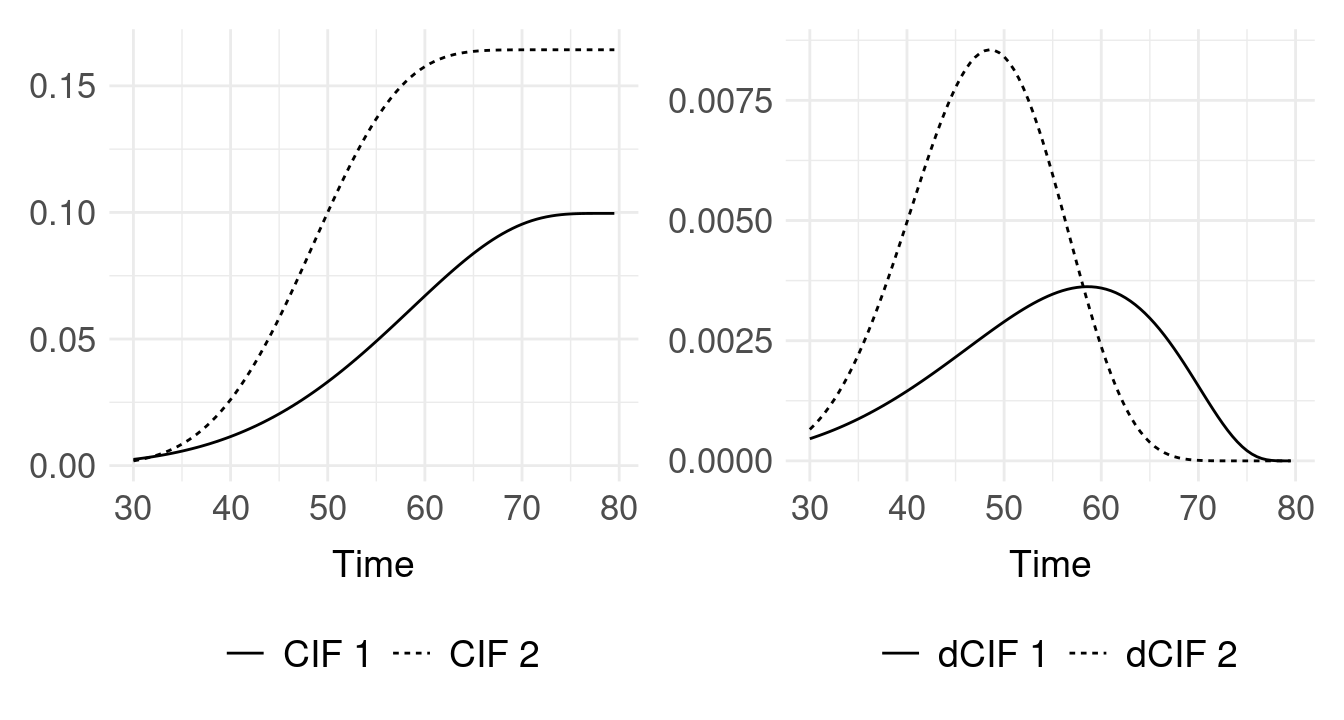
\includegraphics[width=\textwidth]{datasimucif-1.png}
  \\
  \begin{footnotesize}
    SOURCE: The author (2020).
  \end{footnotesize}
  \label{fig:datasimucif}
\end{figure}

By adding the latent structure
\[
  \begin{bmatrix} u_{1}\\u_{2}\\\eta_{1}\\\eta_{2} \end{bmatrix}
  \sim\mathcal{N} \left(
    \begin{bmatrix} 0\\0\\0\\0 \end{bmatrix},
    \begin{bmatrix}
      1&0.4&0.5&0.4\\
      &1&0.4&0.3\\
      &&1&0.4\\
      &&&1
    \end{bmatrix}\right),
\]
in \autoref{eq:modelconfig}, we generate a complete model sample with
500 clusters/pairs of twins, summarized in \autoref{fig:datasimu}.

\begin{figure}[H]
  % \vspace{0.35cm}
  \setlength{\abovecaptionskip}{.0001pt}
  \caption{SUMMARY OF A SIMULATED DATASET WITH 500 PAIRS OF TWINS. A)
    TIME BY TWIN; B) TIMES BOXPLOT; C) PROBABILITIES SCATTERPLOT D)
    \(y_{3}\)'S \%}
  \vspace{0.2cm} \centering
  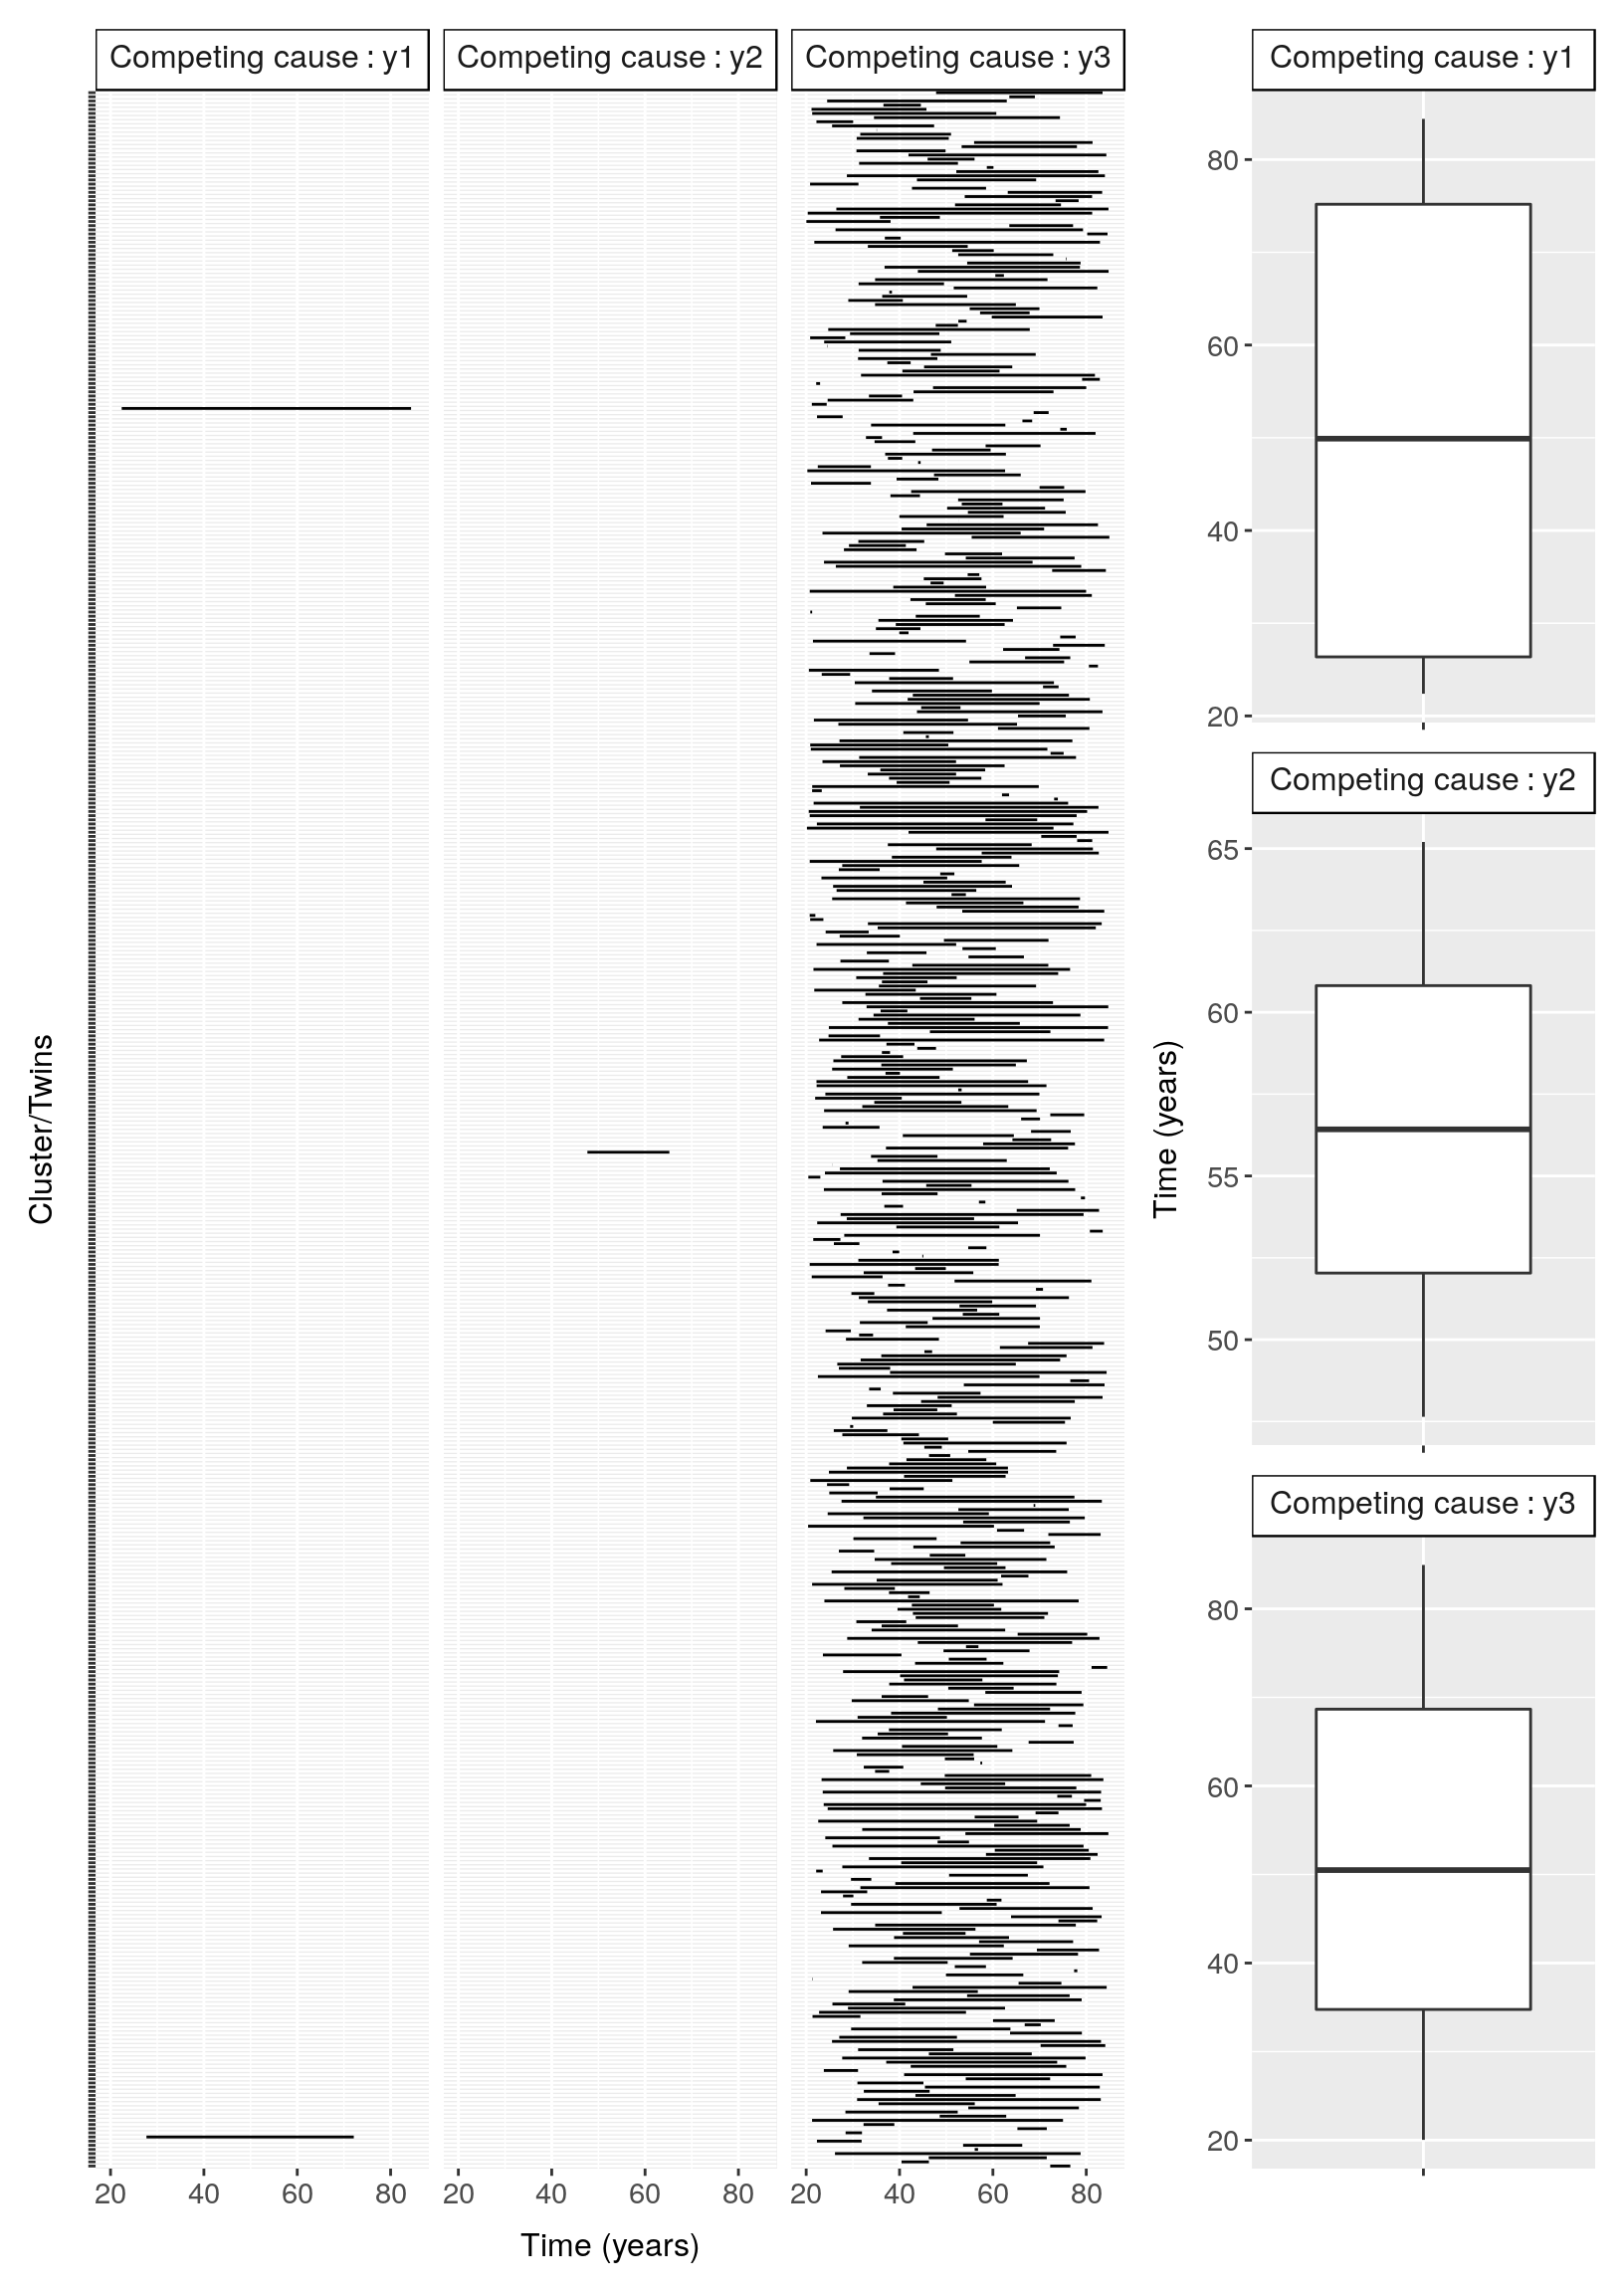
\includegraphics[width=\textwidth]{datasimu-1.png}
  \\
  \vspace{0.2cm}
  \begin{footnotesize}
    SOURCE: The author (2020).
  \end{footnotesize}
  \label{fig:datasimu}
\end{figure}

\section{REAL-BASED DATASET}
\label{cap:data}

% END ==================================================================